\documentclass[12pt,a4paper]{paper}
\usepackage[utf8]{inputenc}
\usepackage[english]{babel}
\usepackage{amsmath}
\usepackage{enumitem}
\usepackage{fixltx2e}
\usepackage{multicol}
\usepackage{amsmath}
\usepackage{enumitem}
\usepackage{arydshln}
\usepackage{amsfonts}
\usepackage{multirow}
\usepackage{multicol}
\usepackage{amssymb}
\usepackage{amsfonts}
\usepackage{amssymb}
\usepackage[left=1cm,right=1cm,top=1.5cm,bottom=2cm]{geometry}
\usepackage{Sweave}
\begin{document}
\title{STAT636 - Homework 4\\\small{Daniel Osorio - dcosorioh@tamu.edu\\Department of Veterinary Integrative Biosciences\\Texas A\&M University}}
\maketitle
\Sconcordance{concordance:HW4_DanielOsorio.tex:HW4_DanielOsorio.Rnw:%
1 17 1 1 0 5 1 1 2 1 0 2 1 3 0 1 2 1 1 1 2 7 0 2 2 7 0 2 2 13 0 1 1 1 4 %
7 0 2 2 7 0 2 2 1 0 2 1 5 0 1 1 6 0 2 2 1 0 2 1 4 0 2 2 6 0 1 1 6 0 1 2 %
3 1 1 2 4 0 1 2 18 1 1 2 1 0 3 1 4 0 1 2 64 1 1 2 1 0 4 1 3 0 1 2 1 1 1 %
2 1 0 1 13 12 0 3 1 4 0 2 2 28 0 2 2 1 0 4 1 26 0 3 1 4 0 1 2 2 1}

\begin{enumerate}
\item Consider the \texttt{wine\_quality\_red} data. Due to privacy and logistic issues, only physicochemical (inputs) and sensory (the output) variables are available (e.g. there is no data about grape types, wine brand, wine selling price, etc.).These contain eleven different variables (1 : fixed acidity; 2 : volatile acidity; 3 : citric acid; 4 : residual sugar; 5 : chlorides; 6 : free sulfur dioxide; 7 : total sulfur dioxide; 8 : density; 9 : pH; 10 : sulphates; 11 : alcohol) and one output (quality (score between 0 and 10) ). Use prcomp to perform principal component analysis.
\begin{Schunk}
\begin{Sinput}
> wqr <- read.csv("winequality_red.csv")
> data <- scale(wqr[,-12], center = TRUE, scale = TRUE)
> pca_data <- prcomp(data)
\end{Sinput}
\end{Schunk}
\begin{enumerate}
\item What proportion of variance is explained by the first principal component? 
\begin{Schunk}
\begin{Sinput}
> summary(pca_data)$importance[2,1]
\end{Sinput}
\begin{Soutput}
[1] 0.28174
\end{Soutput}
\end{Schunk}
\item[] By the second principal component?
\begin{Schunk}
\begin{Sinput}
> summary(pca_data)$importance[2,2]
\end{Sinput}
\begin{Soutput}
[1] 0.17508
\end{Soutput}
\end{Schunk}
\item Compute the Proportion of Variance Explained and Cumulative Proportion of Variance Explained and plot the figures. 
\begin{Schunk}
\begin{Sinput}
> summary(pca_data)$importance
\end{Sinput}
\begin{Soutput}
                            PC1      PC2      PC3      PC4       PC5       PC6
Standard deviation     1.760435 1.387771 1.245208 1.101468 0.9794346 0.8121627
Proportion of Variance 0.281740 0.175080 0.140960 0.110290 0.0872100 0.0599600
Cumulative Proportion  0.281740 0.456820 0.597780 0.708070 0.7952800 0.8552500
                             PC7       PC8       PC9      PC10      PC11
Standard deviation     0.7640623 0.6503512 0.5870623 0.4258323 0.2440457
Proportion of Variance 0.0530700 0.0384500 0.0313300 0.0164800 0.0054100
Cumulative Proportion  0.9083200 0.9467700 0.9781000 0.9945900 1.0000000
\end{Soutput}
\begin{Sinput}
> par(mar=c(3,3,0.5,0.5))
> plot(summary(pca_data)$importance[2,], 
+      xlab = "PC", 
+      ylab = "Proportion of Variance", 
+      las=1, type = "l")
\end{Sinput}
\end{Schunk}
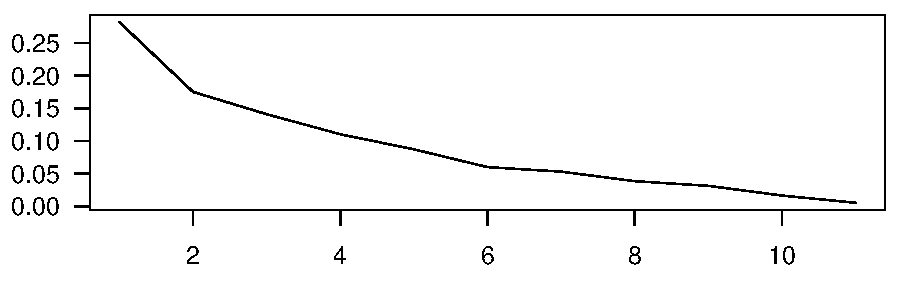
\includegraphics{HW4_DanielOsorio-004}
\item[] How many PCs do you need if you want to capture around 80\% variance?
\begin{Schunk}
\begin{Sinput}
> sum(summary(pca_data)$importance[3,] <= 0.8)
\end{Sinput}
\begin{Soutput}
[1] 5
\end{Soutput}
\end{Schunk}
\item Verify that the variances of the first two PCs equal the first two eigenvalues of the sample covariance matrix \textbf{S}
\begin{Schunk}
\begin{Sinput}
> S <- var(data)
> eS <- eigen(S)
> eS$values[1:2]
\end{Sinput}
\begin{Soutput}
[1] 3.099132 1.925910
\end{Soutput}
\begin{Sinput}
> apply(data %*% eS$vectors,2,var)[1:2]
\end{Sinput}
\begin{Soutput}
[1] 3.099132 1.925910
\end{Soutput}
\end{Schunk}
\item Report a scatterplot of the first two principal components and the first with the third principal components.
\begin{Schunk}
\begin{Sinput}
> par(mfrow=c(1,2), mar=c(4,4,0.5,0.5))
> plot((data %*% eS$vectors)[,c(1,2)], xlab = "PC1", ylab = "PC2", las = 1)
> plot((data %*% eS$vectors)[,c(1,3)], xlab = "PC1", ylab = "PC3", las = 1)
\end{Sinput}
\end{Schunk}
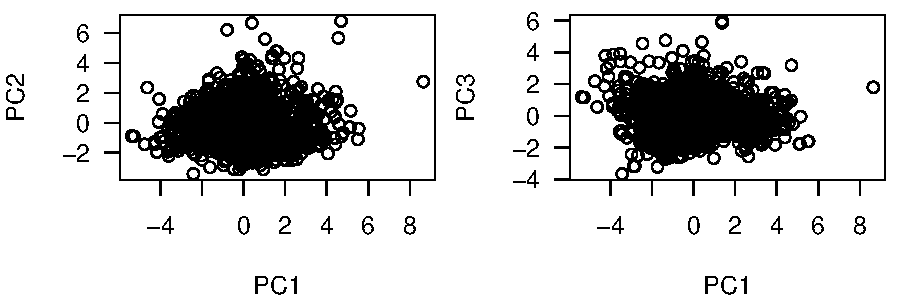
\includegraphics{HW4_DanielOsorio-007}
\item Which number of wine have the minimum and maximum values of PC1?
\begin{Schunk}
\begin{Sinput}
> which.min((data %*% eS$vectors)[,1])
\end{Sinput}
\begin{Soutput}
[1] 1322
\end{Soutput}
\begin{Sinput}
> which.max((data %*% eS$vectors)[,1])
\end{Sinput}
\begin{Soutput}
[1] 152
\end{Soutput}
\end{Schunk}
\end{enumerate}
\item Consider the matrix of distances for four items
\[\left[\begin{array}{cccc}0&&&\\3&0&&\\2&4&0&\\5&1&7&0\end{array}\right]\]
For each of single, complete, and average linkage:
\begin{Schunk}
\begin{Sinput}
> D <- as.dist(matrix(c(0,3,2,5,3,0,4,1,2,4,0,7,5,1,7,0), nrow = 4, byrow = TRUE))
\end{Sinput}
\end{Schunk}
\begin{enumerate}
\item List all intermediate distance matrices involved in the hierarchical clustering routine.
\begin{enumerate}
\item Using single linkage:
\[\left[\begin{array}{cccc}0&&&\\3&0&&\\2&4&0&\\5&\textbf{1}&7&0\end{array}\right] \rightarrow
\left[\begin{array}{ccc}0&&\\3&0&\\4&\textbf{2}&0\end{array}\right] \rightarrow
\left[\begin{array}{cc}0&\\\textbf{3}&0\end{array}\right]\]
\item Using complete linkage:
\[\left[\begin{array}{cccc}0&&&\\3&0&&\\2&4&0&\\5&\textbf{1}&7&0\end{array}\right] \rightarrow
\left[\begin{array}{ccc}0&&\\5&0&\\7&\textbf{2}&0\end{array}\right] \rightarrow
\left[\begin{array}{cc}0&\\\textbf{7}&0\end{array}\right]
\]
\item Using average linkage:
\[\left[\begin{array}{cccc}0&&&\\3&0&&\\2&4&0&\\5&\textbf{1}&7&0\end{array}\right] \rightarrow
\left[\begin{array}{ccc}0&&\\4&0&\\5.5&\textbf{2}&0\end{array}\right] \rightarrow
\left[\begin{array}{cc}0&\\\textbf{4.75}&0\end{array}\right]
\]
\end{enumerate}
\item Draw the dendrograms and compare the results of the different linkage methods.
\begin{Schunk}
\begin{Sinput}
> par(mfrow=c(1,3), mar=c(1,3,1,1))
> plot(hclust(d = D, method = "single"), main = "Single", las=1)
> plot(hclust(d = D, method = "complete"), main = "Complete", las=1)
> plot(hclust(d = D, method = "average"), main= "Average", las=1)
\end{Sinput}
\end{Schunk}
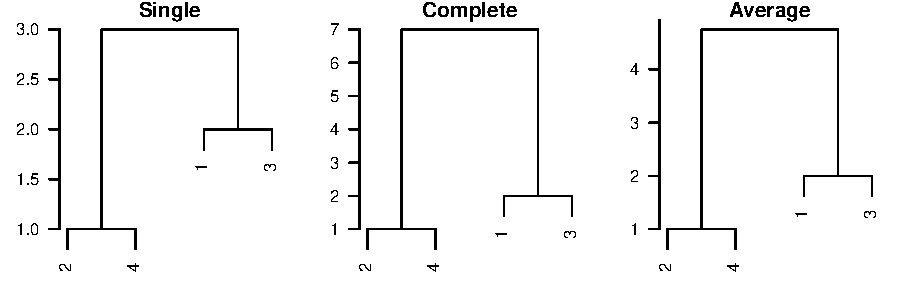
\includegraphics{HW4_DanielOsorio-010}
\end{enumerate}
\item Suppose we measure two variables $X_1$ and $X_2$ for four items $A$, $B$, $C$, and $D$. The data are as follows:
\begin{center}
\begin{tabular}{c|cc}
&\multicolumn{2}{c}{Observations}\\
Item&$x_{1}$&$x_{2}$\\
\hline
A&5&4\\
B&1&-2\\
C&-1&1\\
D&3&1\\
\end{tabular}
\end{center}
\begin{enumerate}
\item Starting with the initial groups (AB) and (CD), write out all steps to the K-means clustering routine with K = 2. Use Euclidean distance on the unstandardized variables.
\begin{enumerate}
\item Compute the coordinates of the cluster centroid (mean)\\
\begin{tabular}{ccc}
&$x_{1}$&$x_{2}$\\
(AB)&3&1\\
(CD)&1&1
\end{tabular}
\item Compute the Euclidean distance of each item from the group centroids and reassign each item to the nearest group.\\
\begin{tabular}{ccc}
&$(AB)$&$(CD)$\\
(A)&\textbf{3.6}&5\\
(B)&3.6&\textbf{3}\\
(C)&4&\textbf{2}\\
(D)&\textbf{0}&2\\
\end{tabular}
\item As two items were moved from the initial configuration,the cluster centroids (means) must be updated.\\
\begin{tabular}{ccc}
&$x_{1}$&$x_{2}$\\
(AD)&4&2.5\\
(BC)&0&-0.5
\end{tabular}
\item Compute the Euclidean distance of each item from the group centroids and reassign each item to the nearest group.\\
\begin{tabular}{ccc}
&$(AD)$&$(BC)$\\
(A)&\textbf{1.8}&6.72\\
(B)&5.4&\textbf{1.8}\\
(C)&5.22&\textbf{1.8}\\
(D)&\textbf{1.8}&3.35\\
\end{tabular}
\end{enumerate}
\item Repeat, now starting with the initial groups (AC) and (BD). Compare the results with those in the part (a).
\begin{enumerate}
\item Compute the coordinates of the cluster centroid (mean)\\
\begin{tabular}{ccc}
&$x_{1}$&$x_{2}$\\
(AC)&2&2.5\\
(BD)&2&-0.5
\end{tabular}
\item Compute the Euclidean distance of each item from the group centroids and reassign each item to the nearest group.\\
\begin{tabular}{ccc}
&$(AC)$&$(BD)$\\
(A)&\textbf{3.35}&5.4\\
(B)&4.6&\textbf{1.8}\\
(C)&\textbf{3.35}&\textbf{3.35}\\
(D)&\textbf{1.8}&\textbf{1.8}\\
\end{tabular}
\item None of the items was reassigned.
\end{enumerate}
\end{enumerate}
\item Consider the \texttt{NCI60} data. This is a cancer cell line microarray data, which consists of 6830 gene expression measurements on 64 cancer cell lines. Each row is a cancer cell line which is labeled with a cancer type (the first column of the data). In what follows, use Euclidean distance on the unstandardized variables.
\begin{Schunk}
\begin{Sinput}
> nci60 <- read.csv("NCI60.csv")
> nci60data <- nci60[2:ncol(nci60)]
> nci60data <- scale(nci60data, center = TRUE, scale = TRUE)
> rownames(nci60data) <- make.unique(as.character(nci60[,1]))
> nci60dist <- dist(nci60data, method = "euclidean")
\end{Sinput}
\end{Schunk}
\begin{enumerate}
\item Carry out complete, average and single linkage hierarchical clustering of the cancer cell line. Report a dendrogram with labels. Which linkage do you like best? Why?
\begin{Schunk}
\begin{Sinput}
> par(mar=c(2,1,1,6), mfrow=c(1,3),mgp=c(2,1,0), cex=0.3)
> plotDendogram <- function(x){
+   result <- hclust(nci60dist, method = tolower(x))
+   par(cex = 0.3)
+   plot(as.dendrogram(result), cex=0.2, horiz = TRUE, 
+        xlab="", ylab="", main="", 
+        sub="", axes=FALSE, xlim = c(160,0))
+   abline(v=(mean(result$height[nrow(result$merge)-c(2,3)])), 
+          lty = 2, 
+          col="red")
+   par(cex=0.5)
+   title(xlab="xlab", ylab="ylab", main=x)
+   axis(1)
+ }
> plotDendogram("Complete")
> plotDendogram("Average")
> plotDendogram("Single")
\end{Sinput}
\end{Schunk}
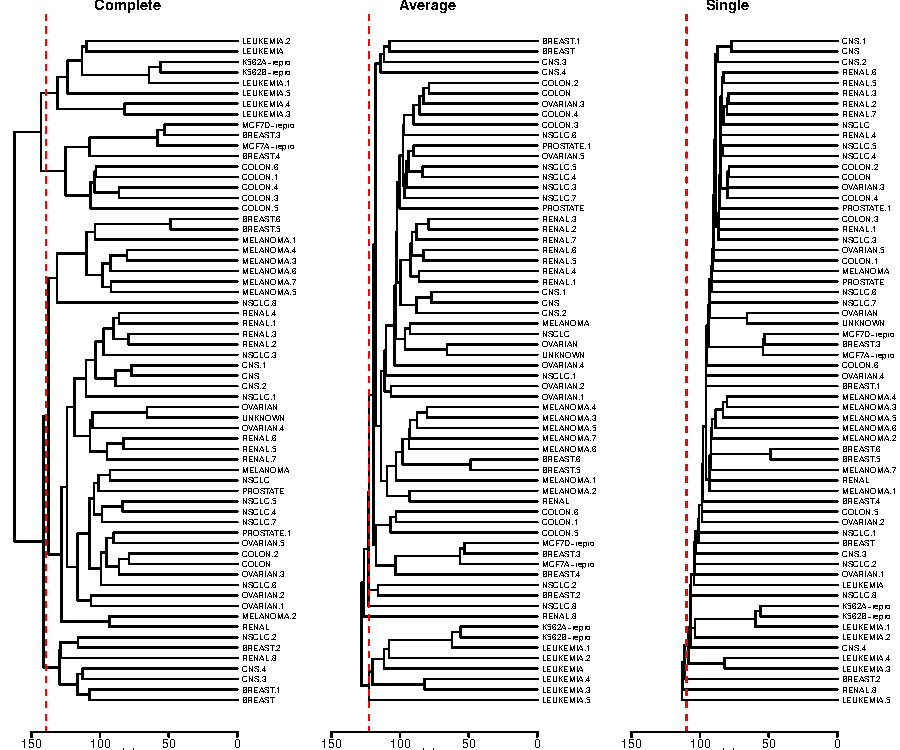
\includegraphics{HW4_DanielOsorio-012}
\item Following we will only use the result getting from complete method. Plot the cut on the dendrogram that produces four clusters and compare the result with the original labels. \textit{Labels are not organized in the same order}. Find one type of cancer fall in one cluster and find one type of cancer spread out over three different clusters. \textit{Breast cancer is present in clusters 2, 1 and 4. Melanoma is only present in cluster 1}
\begin{Schunk}
\begin{Sinput}
> cutree(hclust(nci60dist, method = "complete"),4)[sort(rownames(nci60data))]
\end{Sinput}
\begin{Soutput}
     BREAST    BREAST.1    BREAST.2    BREAST.3    BREAST.4    BREAST.5 
          2           2           2           4           4           1 
   BREAST.6         CNS       CNS.1       CNS.2       CNS.3       CNS.4 
          1           1           1           1           2           2 
      COLON     COLON.1     COLON.2     COLON.3     COLON.4     COLON.5 
          1           4           1           4           4           4 
    COLON.6 K562A-repro K562B-repro    LEUKEMIA  LEUKEMIA.1  LEUKEMIA.2 
          4           3           3           3           3           3 
 LEUKEMIA.3  LEUKEMIA.4  LEUKEMIA.5 MCF7A-repro MCF7D-repro    MELANOMA 
          3           3           3           4           4           1 
 MELANOMA.1  MELANOMA.2  MELANOMA.3  MELANOMA.4  MELANOMA.5  MELANOMA.6 
          1           1           1           1           1           1 
 MELANOMA.7       NSCLC     NSCLC.1     NSCLC.2     NSCLC.3     NSCLC.4 
          1           1           1           2           1           1 
    NSCLC.5     NSCLC.6     NSCLC.7     NSCLC.8     OVARIAN   OVARIAN.1 
          1           1           1           1           1           1 
  OVARIAN.2   OVARIAN.3   OVARIAN.4   OVARIAN.5    PROSTATE  PROSTATE.1 
          1           1           1           1           1           1 
      RENAL     RENAL.1     RENAL.2     RENAL.3     RENAL.4     RENAL.5 
          1           1           1           1           1           1 
    RENAL.6     RENAL.7     RENAL.8     UNKNOWN 
          1           1           2           1 
\end{Soutput}
\end{Schunk}
\item Carry out K-means clustering of the cancer cell lines, with K = 4. Plot the first two principal components and color-code by cluster membership. How do the K-means results compare with the hierarchical clustering results? (Using \texttt{set.seed(2)} before your K-means algorithm and remember scale your data before doing PCA.) \textit{They are not identical but quite similar, Breast cancer is still present in 3 clusters and Melanoma belong to just one.}
\begin{Schunk}
\begin{Sinput}
> pca_nci60 <- eigen(var(nci60data))
> pc_nci60 <- (nci60data %*% pca_nci60$vectors)[,1:2]
> set.seed(2)
> KM <- kmeans(pc_nci60,4)
> KM$cluster[sort(rownames(nci60data))]
\end{Sinput}
\begin{Soutput}
     BREAST    BREAST.1    BREAST.2    BREAST.3    BREAST.4    BREAST.5 
          1           1           1           2           2           4 
   BREAST.6         CNS       CNS.1       CNS.2       CNS.3       CNS.4 
          4           1           1           1           1           1 
      COLON     COLON.1     COLON.2     COLON.3     COLON.4     COLON.5 
          2           2           2           2           2           2 
    COLON.6 K562A-repro K562B-repro    LEUKEMIA  LEUKEMIA.1  LEUKEMIA.2 
          2           3           3           2           3           3 
 LEUKEMIA.3  LEUKEMIA.4  LEUKEMIA.5 MCF7A-repro MCF7D-repro    MELANOMA 
          3           3           2           2           2           1 
 MELANOMA.1  MELANOMA.2  MELANOMA.3  MELANOMA.4  MELANOMA.5  MELANOMA.6 
          4           4           4           4           4           4 
 MELANOMA.7       NSCLC     NSCLC.1     NSCLC.2     NSCLC.3     NSCLC.4 
          4           1           1           1           1           1 
    NSCLC.5     NSCLC.6     NSCLC.7     NSCLC.8     OVARIAN   OVARIAN.1 
          2           2           2           2           1           2 
  OVARIAN.2   OVARIAN.3   OVARIAN.4   OVARIAN.5    PROSTATE  PROSTATE.1 
          1           2           1           1           2           1 
      RENAL     RENAL.1     RENAL.2     RENAL.3     RENAL.4     RENAL.5 
          1           1           1           1           1           1 
    RENAL.6     RENAL.7     RENAL.8     UNKNOWN 
          1           1           1           1 
\end{Soutput}
\begin{Sinput}
> par(mar=c(3,3,1,1))
> plot(pc_nci60, xlab = "PC1", ylab = "PC2")
> points(pc_nci60, col = KM$cluster, pch = 20, cex = 0.8)
\end{Sinput}
\end{Schunk}
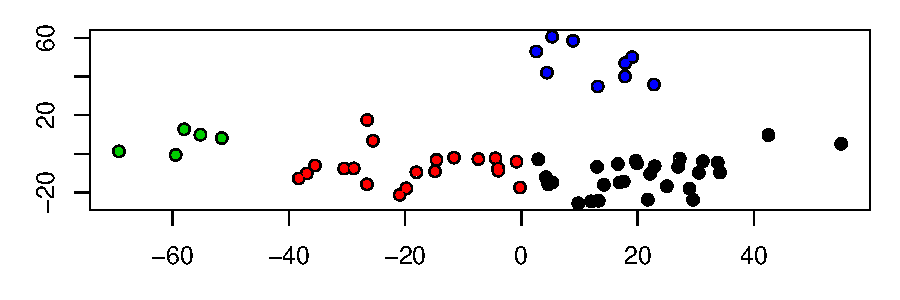
\includegraphics{HW4_DanielOsorio-014}
\end{enumerate}
\end{enumerate}
\end{document}
